%!TEX root = 0.main.tex

\section{How to build a better graph}
Current state of the art: DeepSphere.
Problems: we don't see the convergence expected. in figure \ref{fig:DeepSphere} we see that as $N_{side}$ grows, the eigenspaces of the graph Laplacian do not get more and more aligned with the eigenspaces spanned by the spherical harmonics, as we expected. Why? The parameters to choose are the following: the standard deviation of the Gaussian kernel $t$ and the number of neighbors of the graph. We'll see that the main cause of this bad behavior is the fixed number of neighbors used in \cite{DeepSphere} for the construction of the graph. We'll see that to obtain the desired convergence it is necessary to increase the number of neighbors as we decrease sigma, as we can show hereunder.
\begin{figure}[h]
	\label{fig:DeepSphere}
	\caption{Results from DeepSphere}
	\centering
	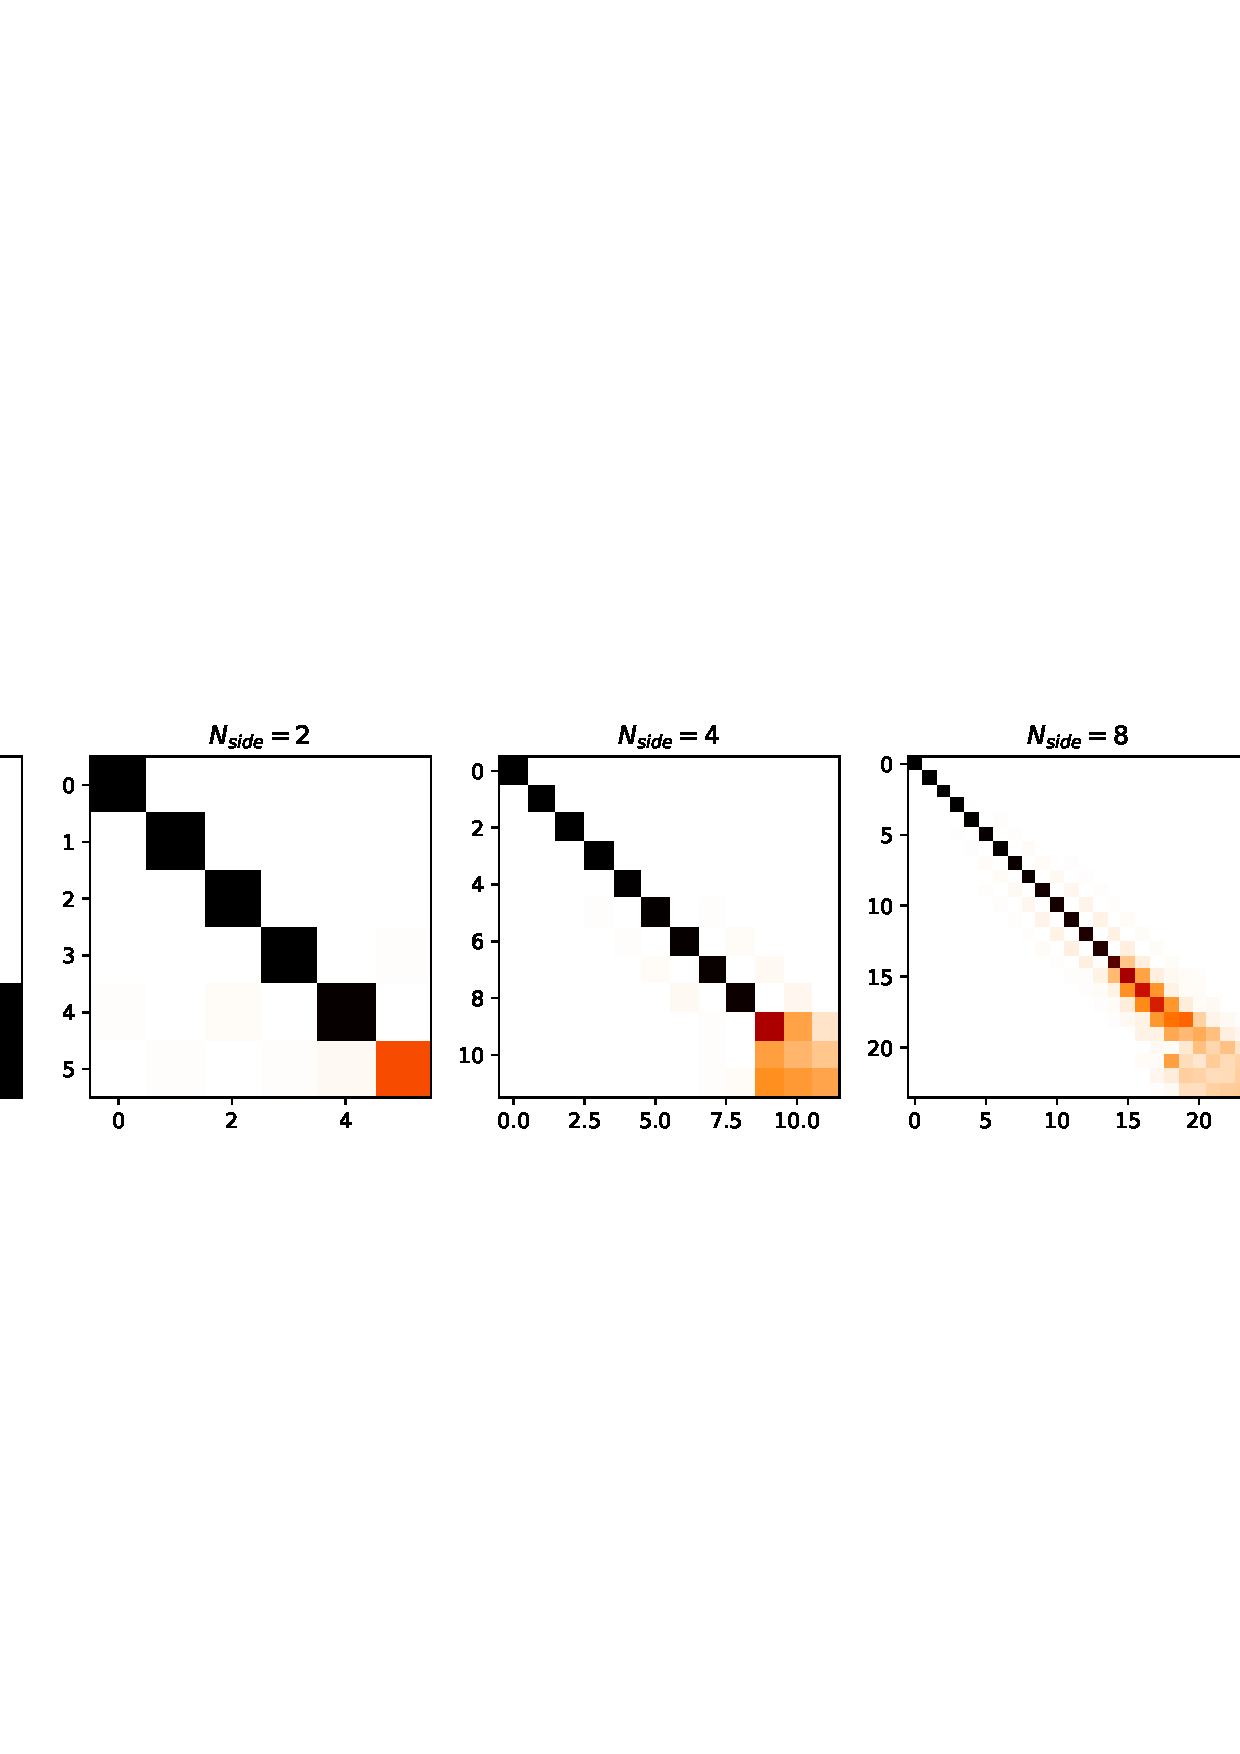
\includegraphics[width=0.9\textwidth]{../codes/06_figures/deepsphere_original.png}
	\includegraphics[width=0.9\textwidth]{../codes/06_figures/deepsphere_original_diagonal.png}	
\end{figure}

\paragraph{Standard deviation of the Gaussian kernel $t$}
Intuition: with a big $t$, the kernel is very wide and the graph can not distinguish the high frequencies. In other words, if we build a radius graph with $d=\bar d$ and connect all the neighbors of a node with the same weights $w$, all the variations on those nodes are indistinguishable. thus, above a certain frequency where the variations reach a wavelength $\omega \leq \bar d$, any graph operator would be blind to such frequencies (indeed, any reordering of the signal on the neighbors would lead to the same result). Thus, if we want our graph Laplacian to be able to distinguish such frequencies, we need our weight to change significantly in a short radius, that means \textbf{setting a $t$ of the order of magnitude of the nearest neighbors of a node}. This intuition was already used in DeepSphere. 

Remember that the convergence result proved in the previous section is valid for a full graph: let's try to see how a full graph built with the same values of $t$ used in \cite{DeepSphere} behaves. 
In figure \ref{fig:DeepSphere_full} we see how for such a full graph it is indeed possible to observe the expected convergence:
\begin{figure}[h]
	\label{fig:DeepSphere_full}
	\caption{DeepSphere \textbf{full}}
	\centering
	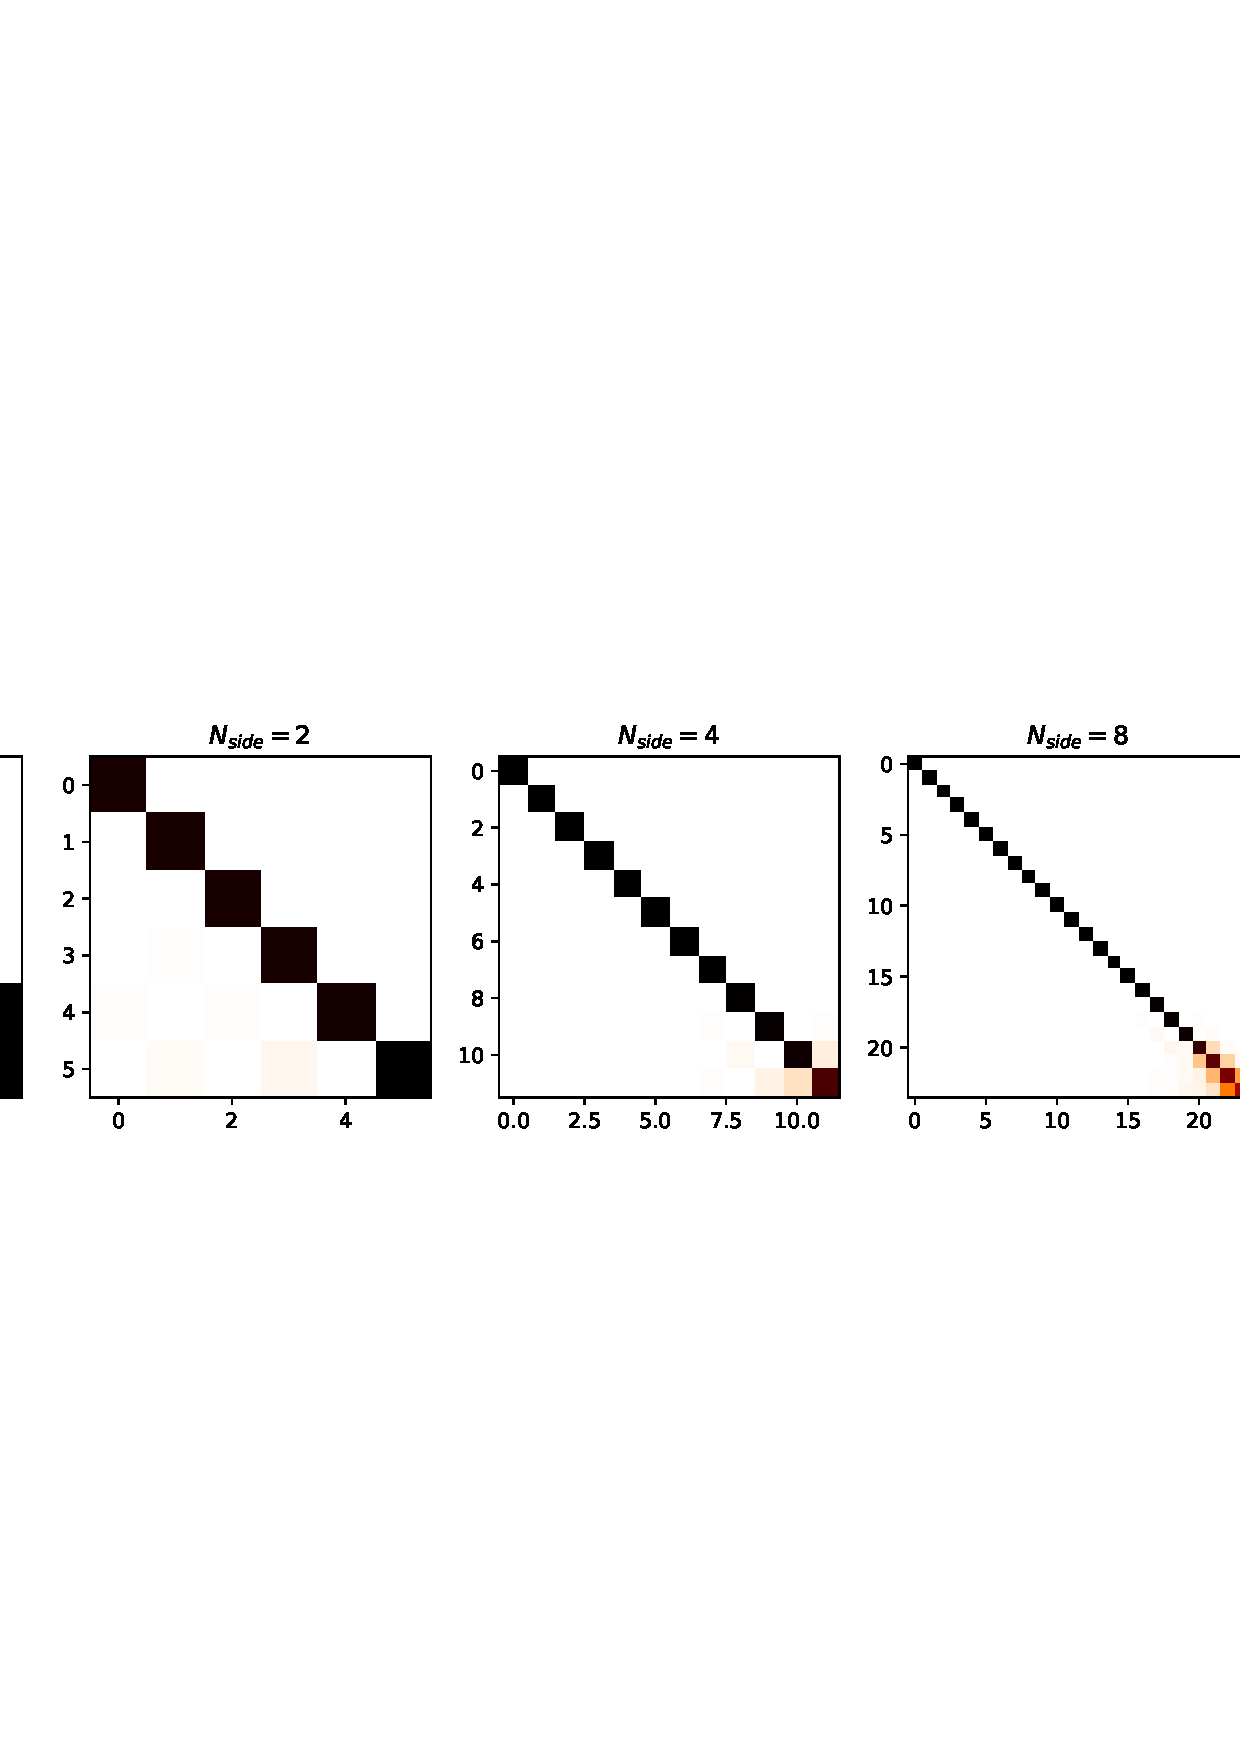
\includegraphics[width=0.9\textwidth]{../codes/06_figures/deepsphere_full.png}
	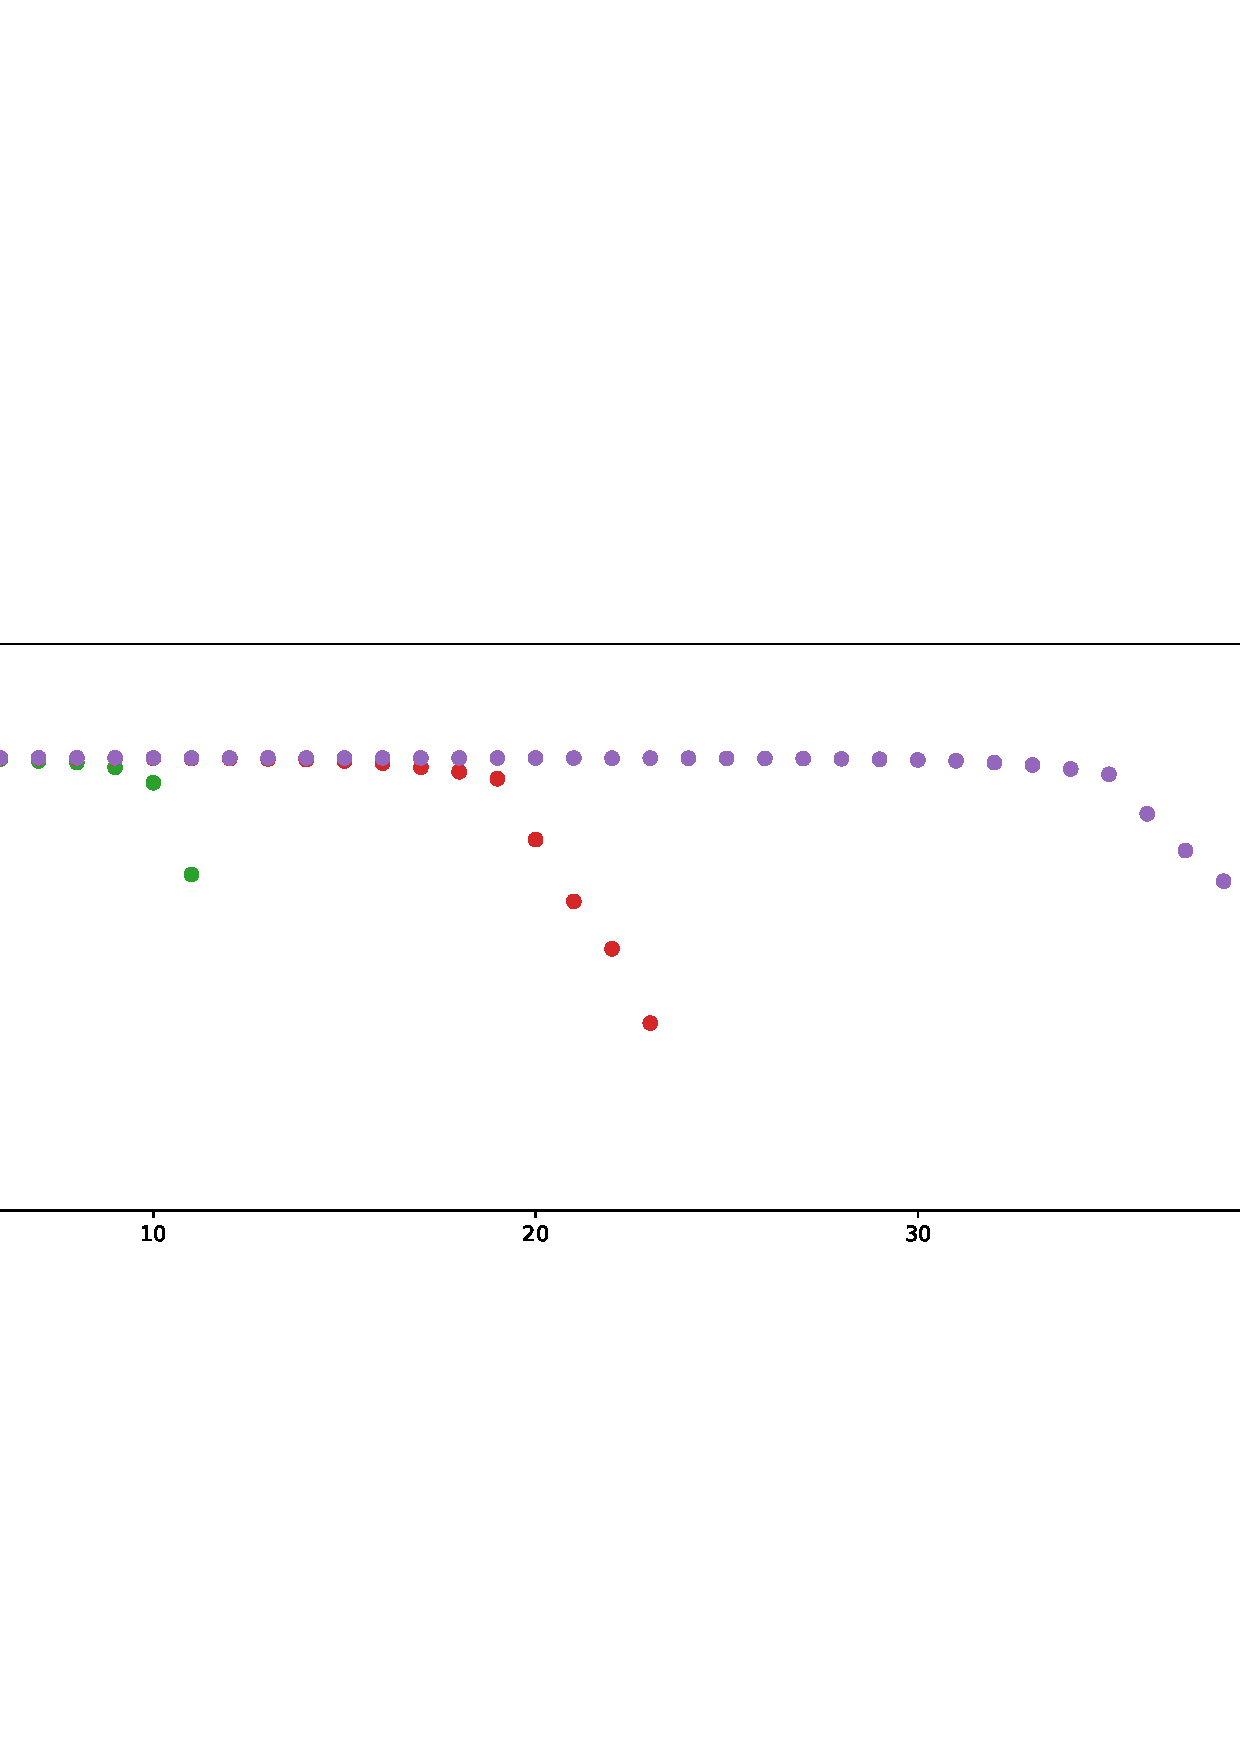
\includegraphics[width=0.9\textwidth]{../codes/06_figures/deepsphere_full_diagonal.png}	
\end{figure}
A quick heuristic grid search has been used to find the following optimal parameters for different values of $N_{side}$ in the case of a full graph. The results are shown in figure \ref{fig:t}. We can see that the heuristic way of \cite{DeepSphere} of setting the standard deviation $t$ produces results very close to the optimal value.

\begin{figure}[h]
	\label{fig:t}
	\caption{Standard deviation of the Gaussian kernel}
	\centering
	\includegraphics[width=0.5\textwidth]{../codes/06_figures/kernelwidth.png}
\end{figure}

However, it is worth showing how the spectrum of the graph is sensible to such parameter. In figure \ref{fig:t_sensitity} it is shown how of the alignment of the eigenspaces is sensible to small changes of $t$. To produce this image $N_{side}$ was set to 16, and a full graph has been build where $t$ has been set first equal to the one used in \cite{DeepSphere} ($t=0.00647$) and then to the optimal value obtained in this work $t=0.015$.

\begin{figure}[h]
	\label{fig:t_sensitity}
	\caption{Standard deviation of the Gaussian kernel}
	\centering
	\includegraphics[width=0.9\textwidth]{../codes/06_figures/t_sensitivity.png}
	\includegraphics[width=0.9\textwidth]{../codes/06_figures/t_sensitivity_diagonal.png}
\end{figure}


\paragraph{Number of neighbors}
For what it concerns the sparsification of the graph, the intuition is the following: remember that we want our graph Laplacian to approximate the operator $L^t$
$$\frac{1}{n}\left(\sum_i e^{-\frac{||x_i-y||}{4t}}(f(y)-f(x_i)) \right) \approx \frac{1}{ 4\pi}\int_\mathcal M e^{-\frac{||x-y||}{4t}}\left(f(y)-f(x)\right)d\mu(x) $$

However, with a full graph the operation of filtering with a polynomial of the graph Laplacian would cost $\mathcal O (n^2)$, same order of magnitude of the method proposed in \cite{bibid}. We want a method to sparsify the graph such that the number of non-null entries of the Laplacian is linear $\mathcal O (n)$, making the filtering operation $f\rightarrow \mathcal P(L)f$ linear in the number of pixels. Deferrard et al. \cite{bibid} fixed the number of neighbors to 7/8. However, their results do not show the expected spectral convergence.
Sparsifing the graph means approximating some weights $w_{i,j}=e^{-\frac{||x_i-x_j||}{4t}} \approx 0$. For this to be accurate we need those weights to be close to 0. A method to be sure that the approximation isn't too bad is the following: \textbf{instead of fixing the number of neighbors, fixing a threshold $k$ on $w_{i,j}=e^{-\frac{||x_i-x_j||}{4t}}$ such that} 
	
$$w_{i,j} = \begin{cases}
e^{-\frac{||x_i-x_j||}{4t}}\quad& \text{if } e^{-\frac{||x_i-x_j||}{4t}} \geq k\\
0 \quad & \text{if } e^{-\frac{||x_i-x_j||}{4t}} < k
\end{cases}$$

By setting $k = 0.01$ here's the result

\begin{figure}[h]
	\label{fig:DeepSphere_thresholded}
	\caption{Deepsphere \textbf{thresholded at $k=0.01$}}
	\centering
	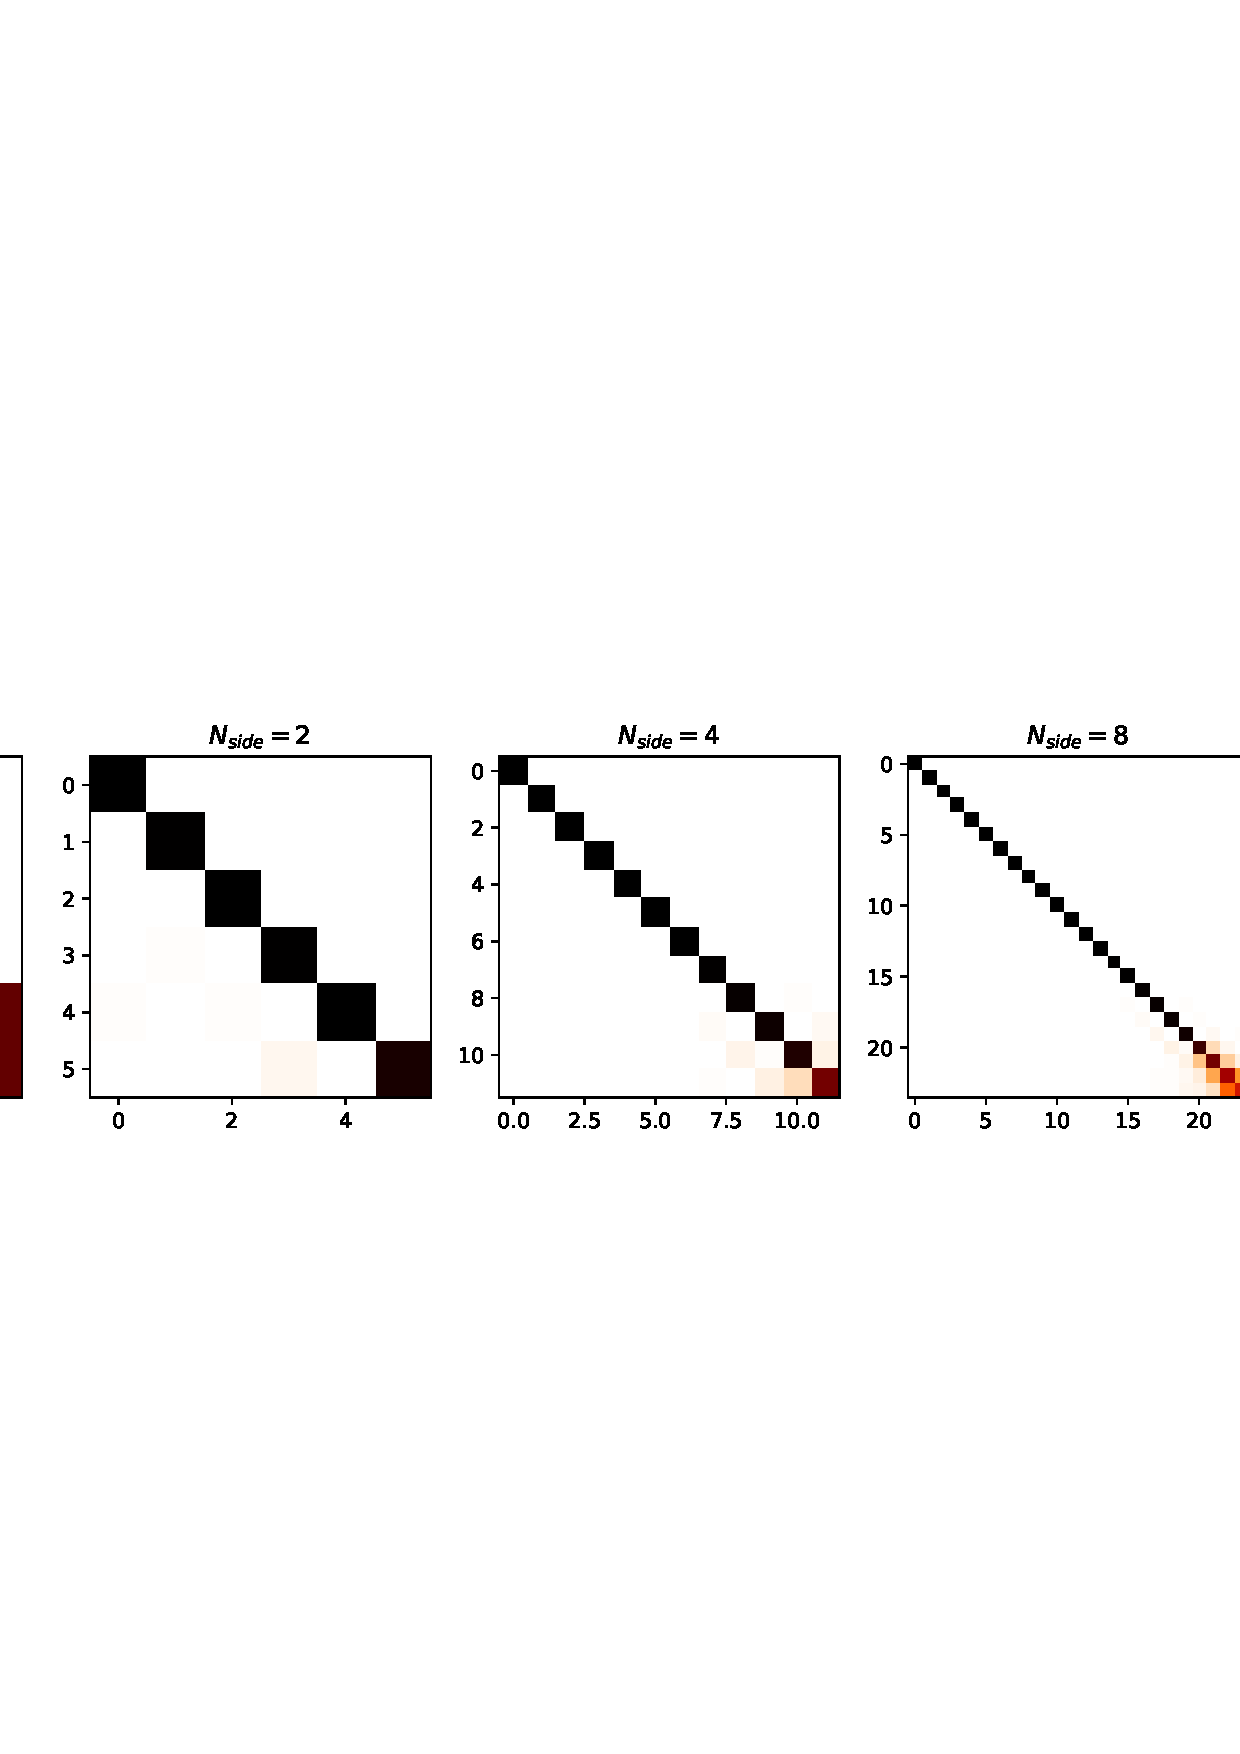
\includegraphics[width=0.9\textwidth]{../codes/06_figures/deepsphere_thresholded.png}	
	\includegraphics[width=0.9\textwidth]{../codes/06_figures/deepsphere_thresholded_diagonal.png}	
\end{figure}

We see that to keep the threshold fixed we need to increase the number of neighbors as $N_{side}$ gets bigger. Again, the intuition is the following: to have spectral convergence (a strong type of convergence) we need more and more global information and more precise.
